\documentclass[11pt,a4paper]{article}
\usepackage[margin=2.2cm]{geometry}
\usepackage{amsmath,amssymb,amsthm,bm,graphicx,booktabs,array,enumitem,xcolor,hyperref,float,tikz}
\usetikzlibrary{positioning,arrows.meta,matrix,fit}
\hypersetup{colorlinks,linkcolor=blue!60!black,urlcolor=blue!60!black}
\newtheorem{definition}{Definition}\newtheorem{lemma}{Lemma}\newtheorem{proposition}{Proposition}\newtheorem{theorem}{Theorem}\newtheorem{remark}{Remark}
\setlength{\parskip}{4pt}
\newcommand{\R}{\mathbb R}\newcommand{\E}{\mathbb E}\newcommand{\Var}{\operatorname{Var}}\newcommand{\Cov}{\operatorname{Cov}}
\title{\vspace{-1.2cm}The paired $t$-test in the approximation study\\[2pt]\large what was tested, how, what it does and does not show}
\author{Note for the paper meeting, 6 November 2026 (Joy)}
\date{}
\begin{document}
\maketitle
\vspace{-0.9cm}
\noindent\textit{Scope.} The differences tables sent to Nadia (\texttt{differences\_KAN\_vs\_MLP}) carry a $t$-statistic and a $p$-value for each comparison. This note states exactly which test produced them (Section~1--2), proves the two facts the test relies on (Section~3), works one comparison through by hand so every printed number can be re-derived (Section~4), gives the full table with two distribution-free checks (Section~5), and lists the assumptions that are and are not met, so the $p$-values are quoted with the right caveats (Section~6). All numbers come from \texttt{differences\_summary\_KAN\_vs\_MLP.csv}; the worked example reproduces the stored $t=-6.4289$, $p=1.58\times10^{-5}$ exactly.

\section{The data structure: 15 cells, each a pair}
For a comparison of model A against model B (e.g.\ A = KAN~[1,1], B = MLP of $t$) the experiment produces, for each asset $a\in\{\text{CBA.AX},\text{TSLA},\text{LLY}\}$ and each budget $N^*\in\{15,30,60,120,240\}$, three fits of A (seeds 0,1,2) and three fits of B (the same seeds). Call the pair $(a,N^*)$ a \emph{cell}; there are $3\times5=15$ cells. Within a cell we form the seed-matched difference and average it over the three seeds:
\begin{equation}
d_{a,N^*}=\frac13\sum_{s=0}^{2}\bigl(\mathrm{RMSE}^{A}_{a,N^*,s}-\mathrm{RMSE}^{B}_{a,N^*,s}\bigr)
=\overline{\mathrm{RMSE}}^{A}_{a,N^*}-\overline{\mathrm{RMSE}}^{B}_{a,N^*}.
\label{eq:d}
\end{equation}
The second equality is just linearity of the mean, so $d$ is the difference of the two cell means that appear in the actual-values table. The same is done for $\max|\mathrm{err}|$ and for fit time. The test is then run on the $n=15$ numbers $d_1,\dots,d_{15}$ (one per cell), and separately per asset on the 5 cells of that asset.

\begin{figure}[H]\centering
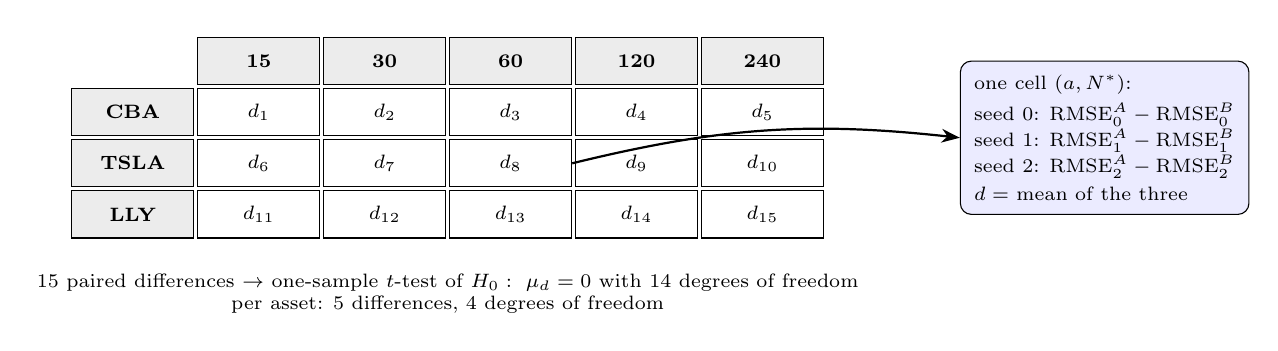
\begin{tikzpicture}[font=\scriptsize,>=Stealth]
\matrix (M) [matrix of nodes,nodes={draw,minimum width=1.55cm,minimum height=6mm,anchor=center},column sep=1pt,row sep=1pt,
 row 1/.style={nodes={fill=gray!15,font=\scriptsize\bfseries}},column 1/.style={nodes={fill=gray!15,font=\scriptsize\bfseries}}]{
   & 15 & 30 & 60 & 120 & 240 \\
 CBA & $d_{1}$ & $d_{2}$ & $d_{3}$ & $d_{4}$ & $d_{5}$ \\
 TSLA & $d_{6}$ & $d_{7}$ & $d_{8}$ & $d_{9}$ & $d_{10}$ \\
 LLY & $d_{11}$ & $d_{12}$ & $d_{13}$ & $d_{14}$ & $d_{15}$ \\};
\node[draw,rounded corners,fill=blue!8,right=1.6cm of M,align=left,inner sep=5pt] (cell) {one cell $(a,N^*)$:\\[2pt]
 seed 0: $\mathrm{RMSE}^A_{0}-\mathrm{RMSE}^B_{0}$\\ seed 1: $\mathrm{RMSE}^A_{1}-\mathrm{RMSE}^B_{1}$\\ seed 2: $\mathrm{RMSE}^A_{2}-\mathrm{RMSE}^B_{2}$\\[2pt] $d=$ mean of the three};
\draw[->,thick] (M-3-4.east) to[bend left=10] (cell.west);
\node[below=2mm of M,align=center]{15 paired differences $\to$ one-sample $t$-test of $H_0:\ \mu_d=0$ with 14 degrees of freedom\\ per asset: 5 differences, 4 degrees of freedom};
\end{tikzpicture}
\caption{The design. A ``pair'' is one model against the other on the same asset, the same budget and the same seeds; the test sees only the 15 cell differences.}
\end{figure}

\begin{figure}[H]\centering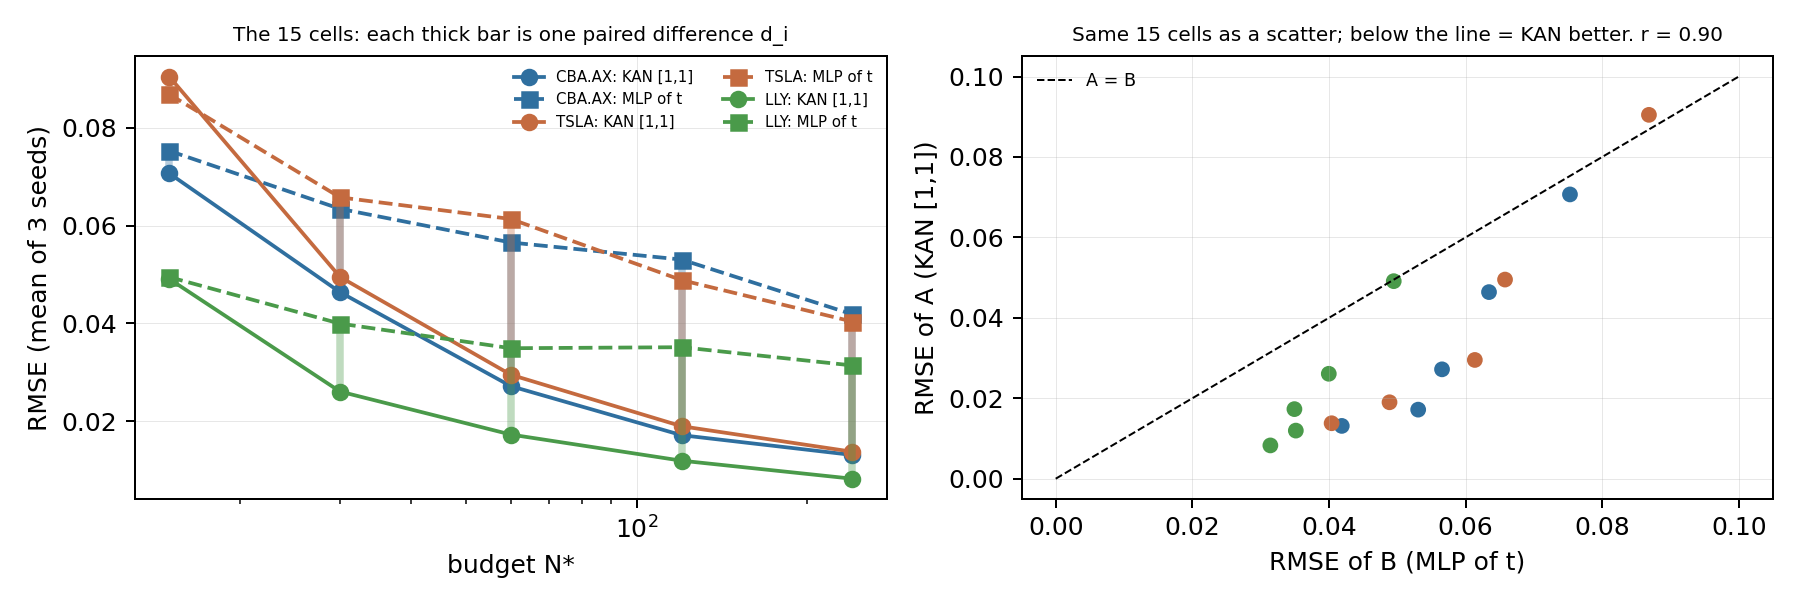
\includegraphics[width=\textwidth]{fig_cells.png}
\caption{KAN~[1,1] vs MLP of $t$, RMSE. Left: the 15 cells, with the paired difference drawn as a thick bar between the two models. Right: the same cells as a scatter of A against B; the strong correlation ($r=0.90$) is what pairing exploits.}
\label{fig:cells}
\end{figure}

\section{The test, precisely}
\begin{definition}[paired $t$-test]
Let $(X_i,Y_i)$, $i=1,\dots,n$, be paired observations and $D_i=X_i-Y_i$. The paired $t$-test of $H_0:\ \E D=0$ against $H_1:\ \E D\neq0$ is the one-sample $t$-test applied to $D_1,\dots,D_n$:
\begin{equation}
\bar D=\frac1n\sum_i D_i,\qquad S_D^2=\frac1{n-1}\sum_i(D_i-\bar D)^2,\qquad T=\frac{\bar D}{S_D/\sqrt n},
\label{eq:T}
\end{equation}
with two-sided $p$-value $p=2\,\Pr(t_{n-1}\ge|T|)$, where $t_{n-1}$ is Student's distribution with $n-1$ degrees of freedom.
\end{definition}
In the code this is literally \texttt{scipy.stats.ttest\_1samp(d, 0.0)} applied to the 15 cell differences (\texttt{differences.py}, lines 68--75), which computes \eqref{eq:T} with $S_D$ using the $n-1$ denominator. Nothing else is done: no pooling of seeds across cells, no variance from the within-cell seed spread, no correction for multiple comparisons. The reported ``mean\_difference'' is $\bar D$, ``t\_statistic'' is $T$, ``p\_value'' is $p$.

\section{Two facts the test rests on}
\begin{theorem}[Student 1908; Fisher 1925]\label{thm:t}
If $D_1,\dots,D_n$ are independent and identically distributed $\mathcal N(\mu,\sigma^2)$, then under $H_0:\mu=0$ the statistic $T$ of \eqref{eq:T} has Student's $t$-distribution with $n-1$ degrees of freedom, whatever the value of $\sigma^2$.
\end{theorem}
\begin{proof}[Proof sketch]
Write $\bm D=(D_1,\dots,D_n)$ and let $\bm 1$ be the all-ones vector. Decompose $\bm D$ into its projection onto $\bm 1$, which is $\bar D\bm 1$, and the orthogonal residual $\bm D-\bar D\bm1$. For a spherical Gaussian vector, orthogonal projections are independent Gaussians; hence $\bar D\sim\mathcal N(0,\sigma^2/n)$ is independent of the residual, and $(n-1)S_D^2/\sigma^2=\|\bm D-\bar D\bm1\|^2/\sigma^2\sim\chi^2_{n-1}$ (Cochran's theorem, the residual lives in an $(n-1)$-dimensional subspace). Then
$T=\dfrac{\bar D/(\sigma/\sqrt n)}{\sqrt{\,[(n-1)S_D^2/\sigma^2]/(n-1)\,}}$ is a standard normal divided by the square root of an independent $\chi^2_{n-1}/(n-1)$, which is the definition of $t_{n-1}$. The unknown $\sigma$ cancels.
\end{proof}
The theorem says \emph{why} the $p$-value is computed from $t_{14}$ and not from a normal curve: with only 15 differences the estimate $S_D$ is noisy, and $t_{14}$ has heavier tails than $\mathcal N(0,1)$ to account for that (the two-sided 5\% critical value is $2.145$ instead of $1.960$). It also lists the assumptions: independence, identical distribution, normality. Section~6 examines each.

\begin{proposition}[why pair]\label{prop:pair}
For paired observations with $\Var X=\sigma_X^2$, $\Var Y=\sigma_Y^2$ and correlation $\rho$,
\[\Var(X-Y)=\sigma_X^2+\sigma_Y^2-2\rho\,\sigma_X\sigma_Y .\]
Hence whenever $\rho>0$ the paired difference has strictly smaller variance than the value $\sigma_X^2+\sigma_Y^2$ that an unpaired comparison of two independent samples would use, and the paired test is correspondingly more powerful; the gain is a factor $1-2\rho\sigma_X\sigma_Y/(\sigma_X^2+\sigma_Y^2)$, which for $\sigma_X\approx\sigma_Y$ is about $1-\rho$.
\end{proposition}
\begin{proof}
$\Var(X-Y)=\Var X+\Var Y-2\Cov(X,Y)$ and $\Cov(X,Y)=\rho\sigma_X\sigma_Y$ by definition of $\rho$. An unpaired two-sample test treats $X$ and $Y$ as independent, i.e.\ uses $\sigma_X^2+\sigma_Y^2$; the paired test uses the true $\Var(X-Y)$, smaller by $2\rho\sigma_X\sigma_Y$.
\end{proof}
In our data (KAN~[1,1] vs MLP of $t$, RMSE) the cell-to-cell spread is large because TSLA is harder than LLY for every model and because every model improves with budget: $\Var A=5.74\times10^{-4}$, $\Var B=2.56\times10^{-4}$, $\rho=0.90$, so $\Var(A-B)=1.40\times10^{-4}$ against $8.30\times10^{-4}$ for the independent-samples assumption, a six-fold reduction. Concretely, an unpaired Welch test on the same 30 numbers gives $t=-2.64$, $p=0.014$; the paired test gives $t=-6.43$, $p=1.6\times10^{-5}$ (Figure~\ref{fig:pairing}). The pairing is not a trick: the two models really were run on the same cells, so their shared difficulty is not evidence either way and should be removed.

\begin{figure}[H]\centering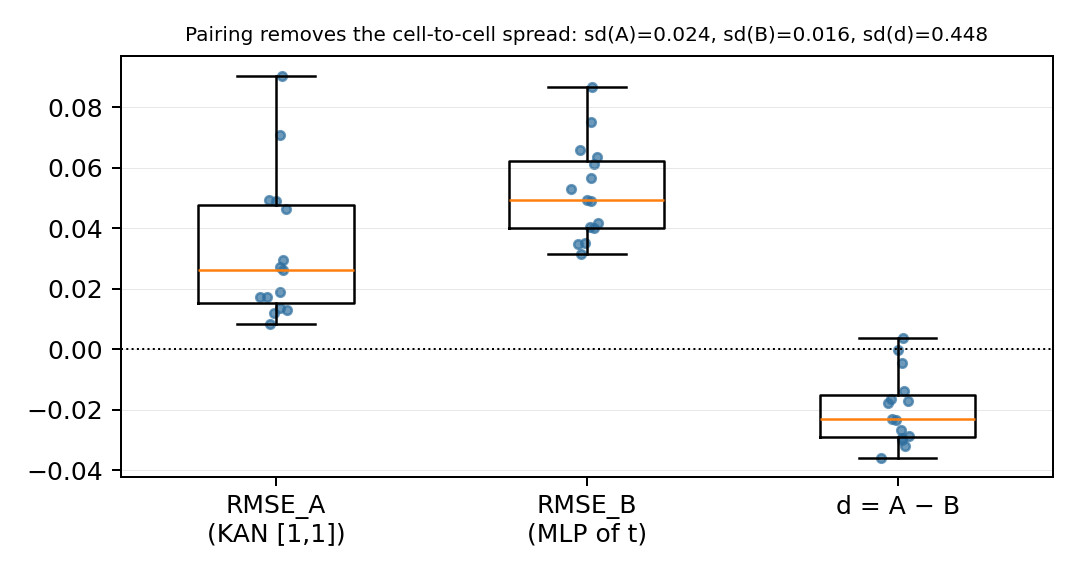
\includegraphics[width=.7\textwidth]{fig_pairing.png}
\caption{Proposition~\ref{prop:pair} in the data: the two models' RMSE values vary a lot across cells (first two boxes) but move together, so their difference (third box) is tight and clearly below zero.}
\label{fig:pairing}
\end{figure}

\section{Worked example: KAN~[1,1] against MLP of $t$, RMSE}
The 15 cell differences $d_i=\overline{\mathrm{RMSE}}^{\text{KAN}}-\overline{\mathrm{RMSE}}^{\text{MLP}}$ (scaled units, from the summary file), ordered CBA, TSLA, LLY and within each by budget:
\begin{center}\small
\begin{tabular}{l@{\hspace{6pt}}rrrrr}
\toprule
 & 15 & 30 & 60 & 120 & 240\\
\midrule
CBA  & $-0.00460$ & $-0.01703$ & $-0.02936$ & $-0.03589$ & $-0.02875$\\
TSLA & $+0.00363$ & $-0.01626$ & $-0.03182$ & $-0.02986$ & $-0.02660$\\
LLY  & $-0.00037$ & $-0.01389$ & $-0.01764$ & $-0.02319$ & $-0.02315$\\
\bottomrule
\end{tabular}
\end{center}
\begin{align*}
\bar D&=-0.019651,& S_D&=0.011838,& \frac{S_D}{\sqrt{15}}&=0.003057,\\
T&=\frac{-0.019651}{0.003057}=-6.429,& p&=2\Pr(t_{14}\ge6.429)=1.58\times10^{-5}.
\end{align*}
A 95\% confidence interval for the mean difference is $\bar D\pm t_{14,0.975}\,S_D/\sqrt n=-0.0197\pm2.145\times0.003057=[-0.0262,\,-0.0131]$: on average over the 15 cells, KAN~[1,1] has an RMSE between $0.013$ and $0.026$ lower (in units where $1$ is the asset's full price range). The standardised effect size (Cohen's $d_z=\bar D/S_D$) is $-1.66$, i.e.\ the mean difference is $1.7$ standard deviations of the differences away from zero; by the usual conventions anything above $0.8$ is ``large''. Fourteen of the fifteen differences are negative; the one positive cell is TSLA at budget~15, where both models are poor ($0.090$ vs $0.087$).

\begin{figure}[H]\centering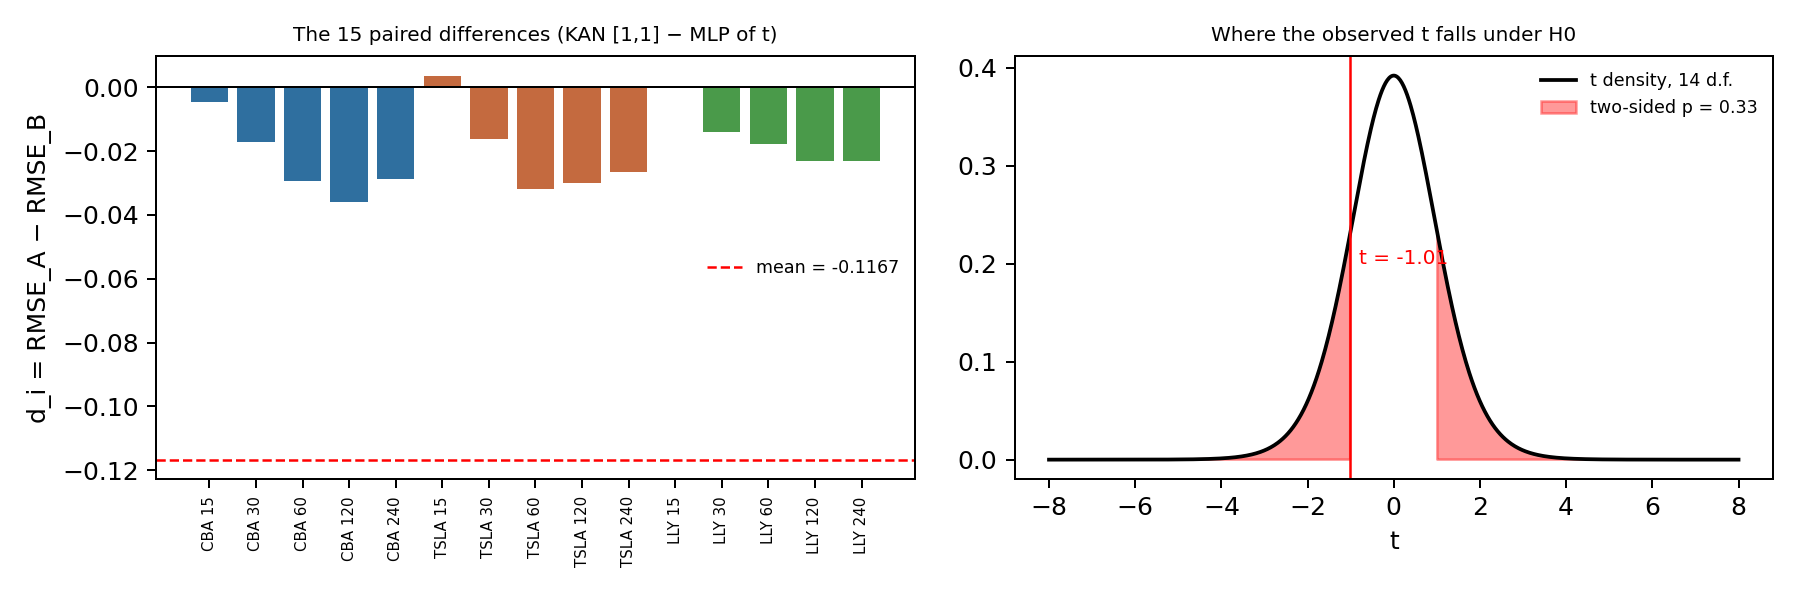
\includegraphics[width=\textwidth]{fig_t.png}
\caption{Left: the 15 differences and their mean. Right: Student's $t_{14}$ density with the observed $T=-6.43$ marked; the shaded two-sided tail area is the $p$-value, far too small to see.}
\end{figure}

\section{All comparisons, with two distribution-free checks}
Because normality and independence are assumptions, each $t$-test was re-done in two ways that need neither: the \emph{Wilcoxon signed-rank test}, which ranks $|d_i|$ and asks whether the ranks of the negative and positive differences are balanced (assumes only a symmetric distribution of $d$ under $H_0$), and the \emph{sign test}, which counts how many of the 15 differences are negative and compares with Binomial$(15,\tfrac12)$ (assumes nothing but $\Pr(d<0)=\tfrac12$ under $H_0$). For the worked example the exact sign-flip permutation test, which enumerates all $2^{15}=32{,}768$ ways of assigning signs to the $|d_i|$, gives $p=6/32768=1.8\times10^{-4}$ (Figure~\ref{fig:perm}).

\begin{table}[H]\centering\footnotesize\setlength{\tabcolsep}{4pt}
\caption{Paired tests on the 15 cell differences (A $-$ B). $d_z=\bar D/S_D$. Negative means A better. ``neg'' = number of the 15 cells with $d<0$.}
\begin{tabular}{llrrrrrrr}
\toprule
comparison (A $-$ B) & metric & $\bar D$ & $S_D$ & $t_{14}$ & $p$ ($t$) & $p$ (Wilcoxon) & neg & $p$ (sign)\\
\midrule
KAN [1,1] $-$ MLP of $t$ & RMSE & $-0.0197$ & $0.0118$ & $-6.43$ & $1.6\times10^{-5}$ & $1.8\times10^{-4}$ & 14 & $0.001$\\
 & max$|$err$|$ & $-0.0615$ & $0.0415$ & $-5.74$ & $5.1\times10^{-5}$ & $1.8\times10^{-4}$ & 14 & $0.001$\\
KAN [1,1] $-$ Fourier MLP & RMSE & $-0.0050$ & $0.0070$ & $-2.79$ & $0.015$ & $0.030$ & 11 & $0.12$\\
 & max$|$err$|$ & $-0.0351$ & $0.0504$ & $-2.69$ & $0.017$ & $0.018$ & 11 & $0.12$\\
KAN [1,$h$,1] $-$ KAN [1,1] & RMSE & $+0.0188$ & $0.0121$ & $+6.04$ & $3.0\times10^{-5}$ & $4.3\times10^{-4}$ & 2 & $0.007$\\
 & max$|$err$|$ & $+0.0585$ & $0.0402$ & $+5.63$ & $6.2\times10^{-5}$ & $3.1\times10^{-4}$ & 1 & $0.001$\\
Fourier MLP $-$ MLP of $t$ & RMSE & $-0.0146$ & $0.0179$ & $-3.16$ & $0.007$ & $0.010$ & 11 & $0.12$\\
 & max$|$err$|$ & $-0.0264$ & $0.0863$ & $-1.18$ & $0.26$ & $0.25$ & 10 & $0.30$\\
\bottomrule
\end{tabular}
\end{table}
Reading across a row: where the $t$-test says ``clearly different'' ($p<10^{-4}$) the rank test agrees, and the crude sign test agrees at the $1\%$ level; where the $t$-test is marginal (KAN~[1,1] vs Fourier MLP, $p\approx0.015$) the sign test, with only 11 of 15 cells, does not reach $5\%$: the two models differ by a small amount that is consistent in direction but not in every cell. Fourier MLP vs MLP of $t$ in max$|$err$|$ is not significant by any test, because the Fourier MLP is worse at the two small budgets and better at the three large ones (Section~6, point 4 of the earlier note). The ``seconds'' rows of the CSV are omitted here on purpose: they compare 80 L-BFGS steps with $20{,}000$ Adam steps and say nothing about the architectures.

\begin{figure}[H]\centering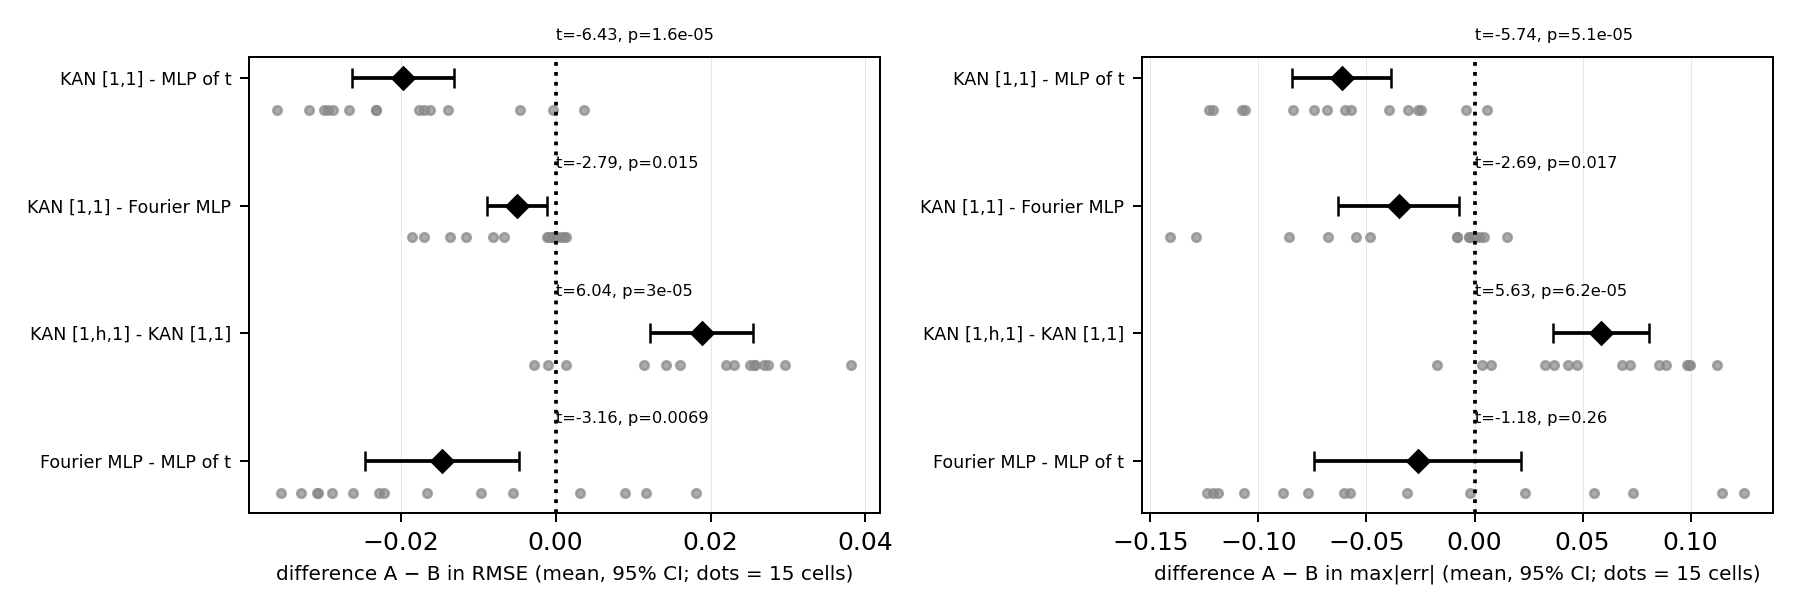
\includegraphics[width=\textwidth]{fig_forest.png}
\caption{All four comparisons: mean difference with 95\% $t$-interval (diamond and bar), the 15 individual cell differences (grey dots), and $t$, $p$. An interval that excludes zero corresponds to $p<0.05$.}
\end{figure}

\begin{figure}[H]\centering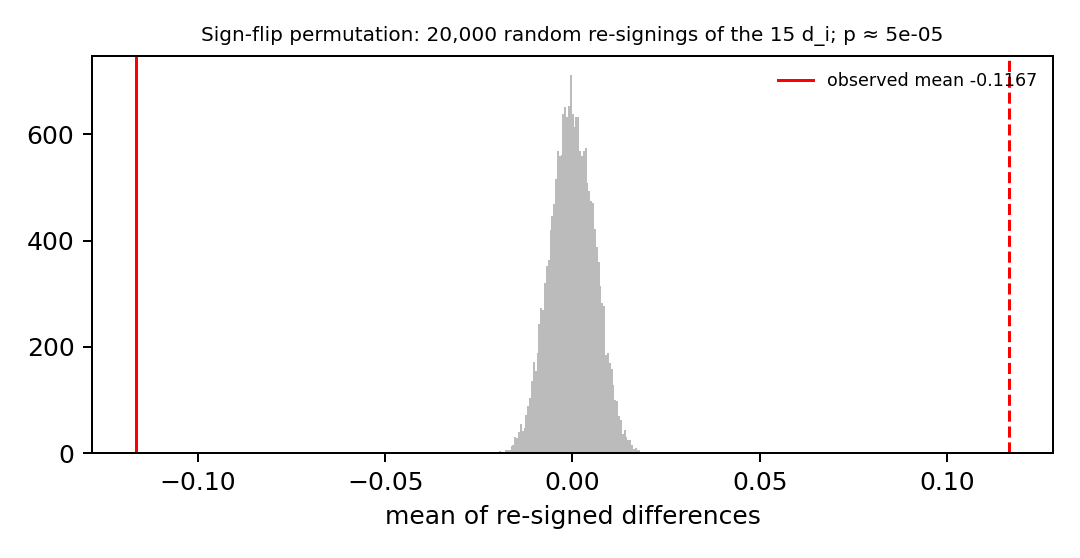
\includegraphics[width=.68\textwidth]{fig_perm.png}
\caption{Exact alternative to Theorem~\ref{thm:t} for the worked example: under $H_0$ each $d_i$ is as likely to be positive as negative, so the null distribution of $\bar D$ can be built by re-signing. Only 6 of the $32{,}768$ sign patterns give a mean as extreme as the observed one.}
\label{fig:perm}
\end{figure}

\section{Assumptions: which hold, which do not, and what that means}
\begin{enumerate}[leftmargin=1.4em,itemsep=3pt]
\item \textbf{Normality of the $d_i$.} Needed for Theorem~\ref{thm:t} exactly; approximately sufficient for $n=15$ by the central limit effect on $\bar D$. A Shapiro--Wilk test on the 15 worked-example differences gives $W=0.93$, $p=0.28$: no evidence against normality, though 15 points cannot show much. The agreement with Wilcoxon and the exact permutation $p$ is the better reassurance.
\item \textbf{Independence of the $d_i$.} This is the assumption that fails, and it is why the $p$-values are described as \emph{descriptive} in the emails and should be in the paper. The 15 cells are not 15 independent draws: (a) the five budgets of one asset are fitted to the \emph{same} 901-point series, and the differences vary smoothly with $N$ (Figure~\ref{fig:depend}); (b) the three assets share the same global market period (2020--2023); (c) for KAN~[1,$h$,1] the budgets 15 and 30 use the \emph{same} fit ($h=1$), so in the KAN~[1,$h$,1]~$-$~KAN~[1,1] comparison two of the ``15'' cells share their A value. Positive dependence makes the effective sample size smaller than 15 and the true standard error larger than $S_D/\sqrt{15}$, so the printed $p$-values are optimistic. They should be read as a summary of how consistently the sign and size of the difference hold up across cells, not as a probability statement about a population of stock series.
\item \textbf{Identical distribution.} The $d_i$ at budget 15 and at budget 240 do not have the same distribution (the former are near zero for everyone, the latter are large), so the ``$\mu_d$'' being tested is an average effect across budgets, not a constant. This is a legitimate quantity to report, but it is why the per-asset and per-budget breakdowns in the Excel file matter more than a single $p$.
\item \textbf{Multiple comparisons.} The CSV reports $4$ comparisons $\times$ $3$ metrics $\times$ (1 pooled $+$ 3 per-asset) $=48$ tests. With a Bonferroni correction over the 8 architecture-relevant pooled tests in the table above, the threshold for $5\%$ becomes $0.05/8=0.006$: the four comparisons with $p<10^{-4}$ survive easily, Fourier MLP vs MLP of $t$ (RMSE, $p=0.007$) is borderline, and the two KAN~[1,1] vs Fourier MLP results ($p\approx0.015$) do not survive. That is the honest reading: KAN~[1,1] and the Fourier MLP are not distinguishable at matched parameters on this evidence.
\item \textbf{What the test does \emph{not} do.} It does not use the within-cell seed spread (the sd over seeds in the Excel file). An alternative would be to test the 45 per-seed differences directly, which gives $t=-10.6$, $p\approx10^{-13}$ for the worked example, but that treats seeds as independent replicates of the \emph{cell} and inflates the evidence (pseudo-replication: three seeds on the same data are not three new data sets). Averaging over seeds first, as we do, is the conservative choice.
\item \textbf{Effect size over $p$-value.} With $n=15$ a $p$-value is a blunt instrument; the quantities to carry into the paper are the mean difference with its interval and $d_z$. For KAN~[1,1] vs MLP of $t$: $-0.020\ [-0.026,-0.013]$, $d_z=-1.7$; for KAN~[1,$h$,1] vs KAN~[1,1]: $+0.019\ [+0.012,+0.025]$, $d_z=1.6$; for KAN~[1,1] vs Fourier MLP: $-0.005\ [-0.009,-0.001]$, $d_z=-0.7$.
\end{enumerate}

\begin{figure}[H]\centering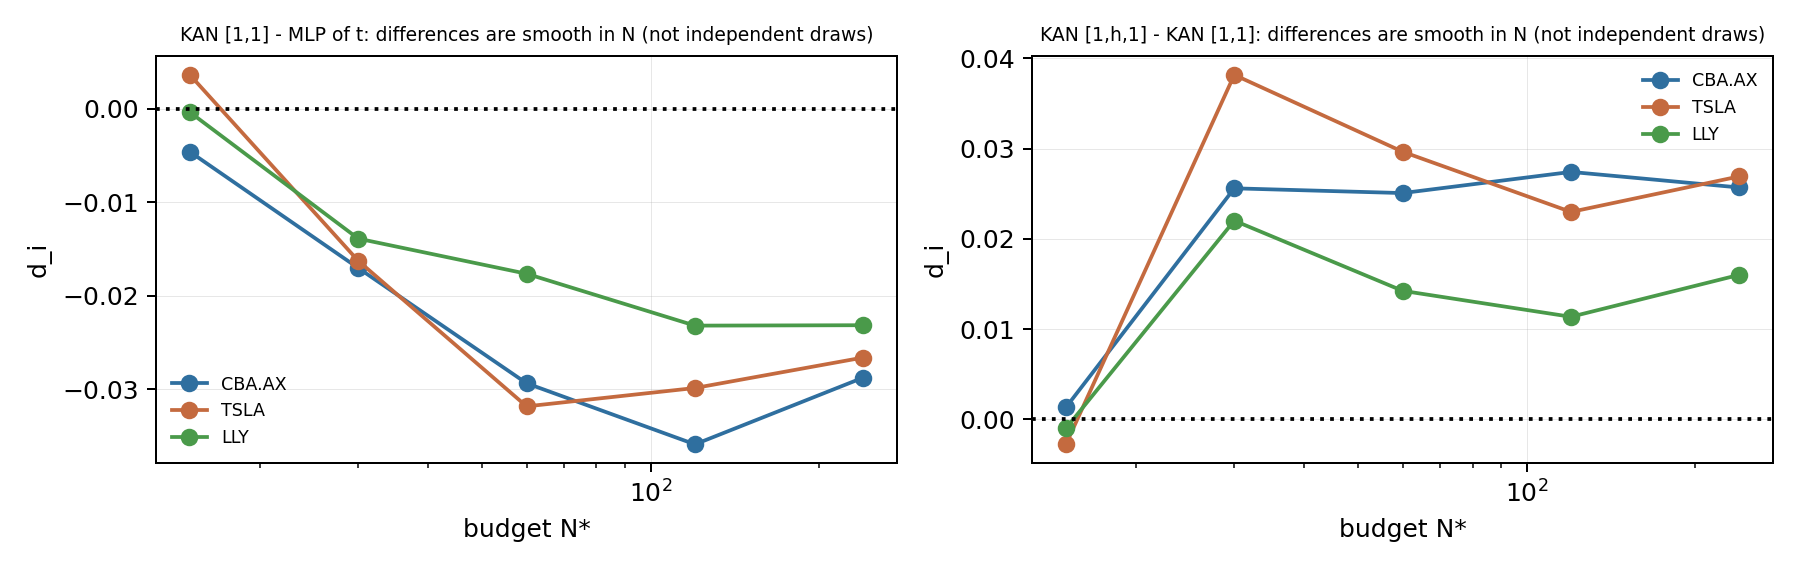
\includegraphics[width=\textwidth]{fig_depend.png}
\caption{Why independence fails: within each asset the five differences trace a smooth curve in the budget, because they come from the same series at increasing resolution. The $t$-test treats these points as unrelated draws.}
\label{fig:depend}
\end{figure}

\section{One sentence for the paper}
``For each comparison a paired $t$-test was applied to the 15 cell differences (three assets $\times$ five budgets, each the mean over three seeds); because the cells share series and are nested in budget, the resulting $p$-values are reported as descriptive summaries of consistency rather than as inferential statements, and are accompanied by the mean difference with its 95\% interval. A Wilcoxon signed-rank test gave the same conclusions in every case.''

\paragraph{References.}
Student (W.~S.~Gosset), The probable error of a mean, \emph{Biometrika} 6 (1908) 1--25.\
R.~A.~Fisher, Applications of ``Student's'' distribution, \emph{Metron} 5 (1925) 90--104.\
W.~G.~Cochran, The distribution of quadratic forms in a normal system, \emph{Proc.\ Cambridge Phil.\ Soc.} 30 (1934) 178--191.\
F.~Wilcoxon, Individual comparisons by ranking methods, \emph{Biometrics Bulletin} 1 (1945) 80--83.\
J.~Cohen, \emph{Statistical Power Analysis for the Behavioral Sciences}, 2nd ed., 1988.\
S.~H.~Hurlbert, Pseudoreplication and the design of ecological field experiments, \emph{Ecological Monographs} 54 (1984) 187--211.\
T.~G.~Dietterich, Approximate statistical tests for comparing supervised classification learning algorithms, \emph{Neural Computation} 10 (1998) 1895--1923.\
J.~Dem\v{s}ar, Statistical comparisons of classifiers over multiple data sets, \emph{JMLR} 7 (2006) 1--30.
\end{document}
